\documentclass[11pt,a4paper]{article}

\usepackage[margin=2.5cm]{geometry}
\usepackage{amsmath}
\usepackage{booktabs}
\usepackage{graphicx}
\usepackage{hyperref}
\usepackage{enumitem}
\usepackage{parskip}
\usepackage{fancyhdr}
\usepackage{float}

\hypersetup{colorlinks=true, linkcolor=blue, urlcolor=blue}
\setlength{\headheight}{14pt}
\pagestyle{fancy}
\fancyhf{}
\lhead{Probe Detection with Deep Learning}
\rfoot{\thepage}

\title{\textbf{Probe Detection with Deep Learning}}
\author{Candidate Assignment Report}
\date{August 2026}

\begin{document}
\maketitle

\begin{abstract}
This project detects an ultrasonic thickness-measurement probe in Elios3 drone images and reports when no probe is detected. The final system is a fine-tuned YOLOv8n detector. The main design work was preventing leakage between similar flight frames, adding a practical no-probe class to a dataset that contains none, and selecting a model that is accurate while suitable for edge deployment.
\end{abstract}

\section{Problem and exploratory data analysis}

The task requires detecting the bounding box of an ultrasonic thickness-measurement probe in images captured by an Elios3 drone, or signaling when no probe is present.

The dataset comprises \textbf{308 grayscale images} ($640\times400$ px) from \textbf{5 drones} and \textbf{21 flight sequences}, each containing one probe annotation in COCO format ($[x, y, w, h]$). Exploratory data analysis (Figure~\ref{fig:dataset_stats}) highlights two key geometric properties: (1) probe boxes are medium-to-large objects (averaging $\approx 125\times 170$ px, aspect ratio $w/h \approx 0.7$), making them well-suited for standard detection heads without multi-scale pyramidal overhead; and (2) probe centers follow a strict bimodal vertical clustering ($y \approx 0.25$ and $y \approx 0.85$), directly reflecting the fixed top/bottom mechanical mounting brackets on the Elios3 frame. Crucially, the dataset contains zero negative (probe-free) images, which must be addressed for practical deployment.

\begin{figure}[H]
\centering
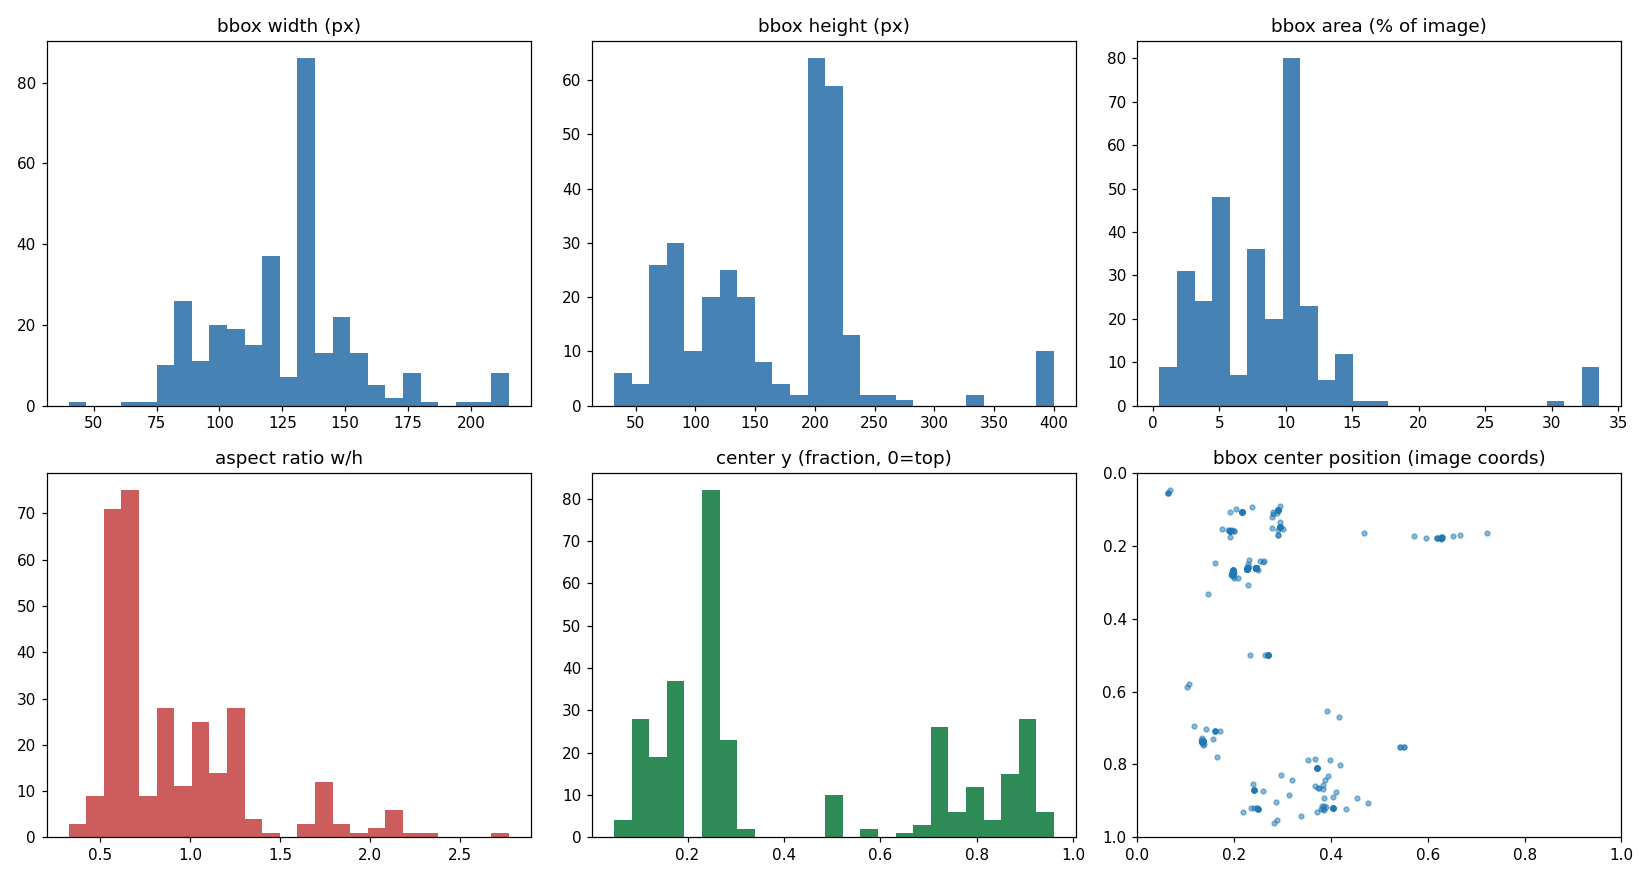
\includegraphics[width=0.75\linewidth]{figures/dataset_stats.png}
\caption{Dataset statistics: bounding-box dimensions, aspect ratio, and bimodal vertical clustering of probe centers.}
\label{fig:dataset_stats}
\end{figure}

\section{Approach}

\subsection{Train/validation/test split}

The data was split by \textbf{drone and flight sequence}, not image by image. Consecutive frames from a sequence have nearly identical background, lighting and probe pose; a random image split would therefore place near-duplicates in both train and test and produce overly optimistic results.

The resulting group-stratified split assigns entire flight sequences to a single partition:
\begin{itemize}[nosep]
    \item \textbf{Train} (213 images, 16 flights): all 5 drones.
    \item \textbf{Validation} (51 images, 4 flights): 3 drones (PREMP00002, SA23130257, 858804493).
    \item \textbf{Test} (44 images, 3 flights): 2 drones (SA22440034, SA22440035) --- held out entirely from validation to avoid selection bias.
\end{itemize}
Validation was used to compare models and choose the confidence threshold; the test set was evaluated only once after those choices were fixed.

\subsection{No-probe examples}\label{sec:no_probe}

Because every raw image contains a probe, synthetic negatives were created by masking the annotated probe region with a small padding and filling it using LaMa generative inpainting. This preserves the full fisheye frame, illumination and scene layout, unlike a resized crop that would change the deployment input distribution. Classical \texttt{cv2.inpaint} was tried first but created visibly blurred fills for large probe regions, so it was not used.

\begin{figure}[H]
\centering
\includegraphics[width=0.75\linewidth]{../data_prep/negatives_qa/all_pairs/050_score-00.325_E300SA23130257_00267_199_1flight_5100_2_neg.jpg}
\caption{Representative synthetic negative: original frame on the left and LaMa-filled frame on the right. The overlay reports this candidate's quality score for QA review.}
\end{figure}

For the experiment reported here, validation and test received one synthetic negative per positive image, allowing measurement of false positives. Training used 64 negatives for 213 positives (30\%): negatives teach object absence but have no box-regression target, so a 1:1 training ratio would reduce the frequency of localization examples. The generation pipeline stores a quality score for each fill: it is the ratio between block-median Laplacian variance inside the filled region and in a surrounding context ring. A value close to 1 means that the fill has similar sharpness to its local background; when selecting a ratio of cached candidates, the smallest $|\mathrm{score}-1|$ values are retained. This is a QA heuristic rather than a ground-truth measure of realism. Real probe-free frames remain the most important future improvement.

\subsection{Model and training}

YOLOv8 was chosen because it offers a robust fine-tuning and export workflow and is appropriate for a small dataset and eventual Jetson-class deployment. Transformer detectors were deliberately not used: with only 308 images their additional capacity is likely overkill, while their larger computational cost works against an edge-device target. The companion edge benchmark (Alqahtani et al., arXiv:2409.16808) also reports YOLOv8 as a strong accuracy/runtime trade-off on Jetson Orin Nano. COCO-pretrained YOLOv8n, YOLOv8s and YOLOv8m were fine-tuned on a Google Colab GPU under the same settings:

\begin{itemize}[nosep]
    \item maximum 100 epochs, early stopping patience 20;
    \item batch size 16 and input size $640\times640$;
    \item Ultralytics Auto optimizer (AdamW, learning rate about 0.002);
    \item default YOLOv8 augmentation: horizontal flip probability 0.5, mosaic and HSV augmentation;
    \item fixed seed 42.
\end{itemize}

No crop-based negative augmentation was used, relying solely on the full-frame inpainted negatives described in Section~\ref{sec:no_probe}. Crops could still be tested later as additional hard negatives, but not as a replacement for full-frame negatives.

No broad hyperparameter search was run. With only about 210 training positives, repeatedly tuning to a small validation set would be more likely to overfit the evaluation than to find a robust improvement. The controlled experiment was model capacity: nano, small and medium were trained identically.

\section{Model selection and evaluation}

The evaluation protocol in \texttt{evaluate.py} measures positive images using IoU, precision, recall, F1, and AP@0.5, and synthetic negative images using the false-positive (FP) rate. Each metric reflects a distinct operational requirement: \textbf{Mean IoU} measures spatial localization accuracy for thickness measurement; \textbf{Precision} prevents false alarms (confusing background structures with probes); \textbf{Recall} ensures probes are not missed during inspection flights; \textbf{F1} and \textbf{AP@0.5} provide balanced overall detection benchmarks; and the \textbf{FP rate} on synthetic negatives directly evaluates no-probe discrimination.

The FP-rate-vs-threshold curve answers: ``if an image contains no probe, how often does the model still report one at this confidence threshold?'' Raising the threshold reduces false positives but can also lower recall on real probes. The validation curve was used to select an operating threshold targeting a 5\% FP rate. Runtime is measured on CPU with batch size 1.

\begin{table}[H]
\centering
\small
\begin{tabular}{lrrrr}
\toprule
Model (validation) & AP@0.5 & F1 & Recall at 5\% FP target & CPU ms/image \\
\midrule
COCO YOLOv8n, no fine-tuning & 0.129 & 0.092 & 0.000 & 141.3 \\
YOLOv8n & \textbf{0.964} & \textbf{0.970} & \textbf{0.961} & \textbf{135.5} \\
YOLOv8s & 0.869 & 0.882 & 0.647 & 280.7 \\
YOLOv8m & 0.732 & 0.767 & 0.647 & 645.4 \\
\bottomrule
\end{tabular}
\caption{Validation comparison. YOLOv8n is both the most accurate and the fastest model on this dataset.}
\end{table}

\begin{figure}[H]
\centering
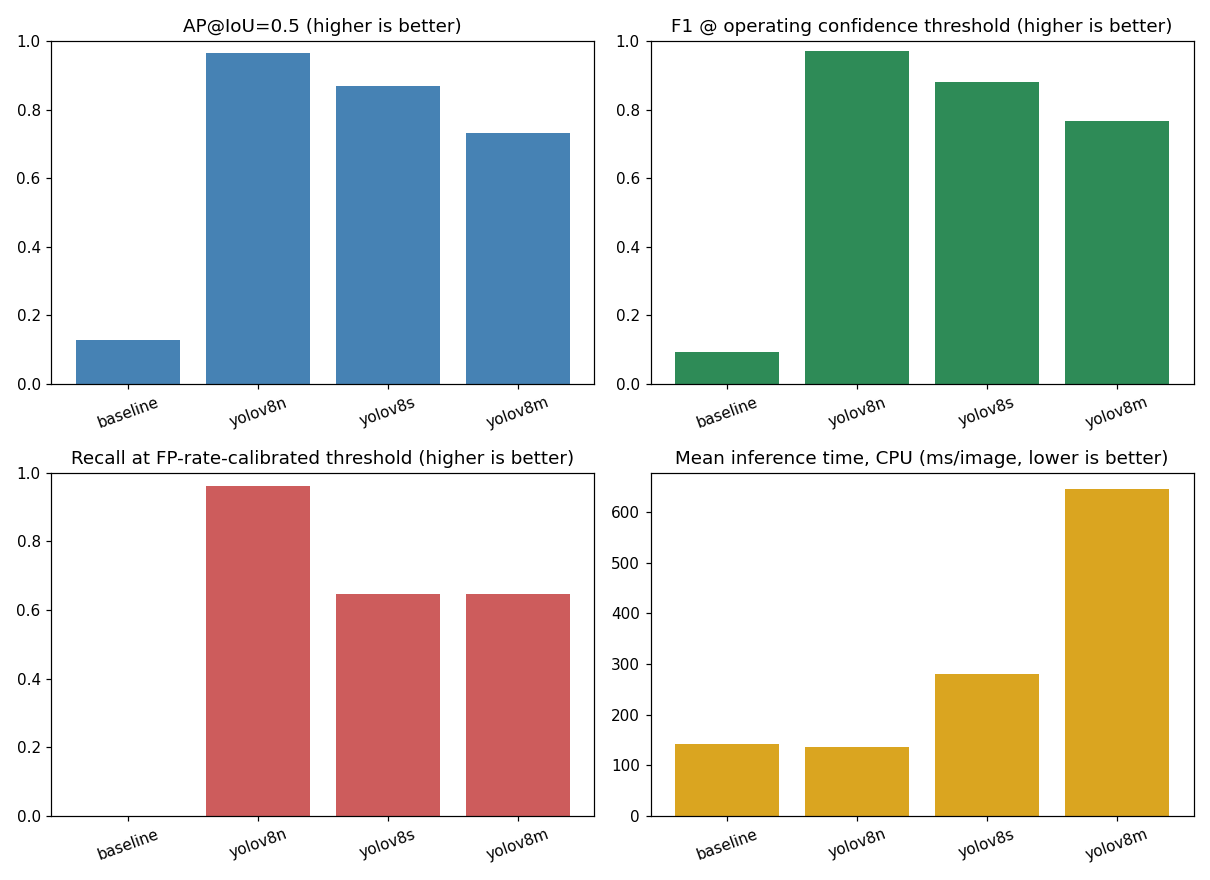
\includegraphics[width=0.52\linewidth]{figures/model_comparison.png}
\caption{Validation comparison of baseline and fine-tuned YOLOv8 variants.}
\end{figure}

YOLOv8n was selected. The larger variants did not benefit from their additional capacity, which is consistent with the limited number of independent training groups.

\begin{table}[H]
\centering
\small
\begin{tabular}{lr}
\toprule
Final held-out test metric (YOLOv8n) & Value \\
\midrule
Positive images / synthetic negatives & 44 / 44 \\
Mean IoU & 0.762 \\
AP@0.5 & 0.951 \\
Chosen default operating threshold ($\tau$) & \textbf{0.22} \\
Recall at operating threshold $\tau = 0.22$ & \textbf{0.886} \\
False-positive rate on negatives ($\tau = 0.22$) & \textbf{0.045} ($<5\%$) \\
Precision / recall / F1 at conservative threshold $\tau = 0.35$ & 0.949 / 0.841 / 0.892 \\
CPU latency / throughput & 98.9 ms / 10.1 FPS \\
\bottomrule
\end{tabular}
\caption{One-time evaluation on the held-out test split.}
\end{table}

\begin{figure}[H]
\centering
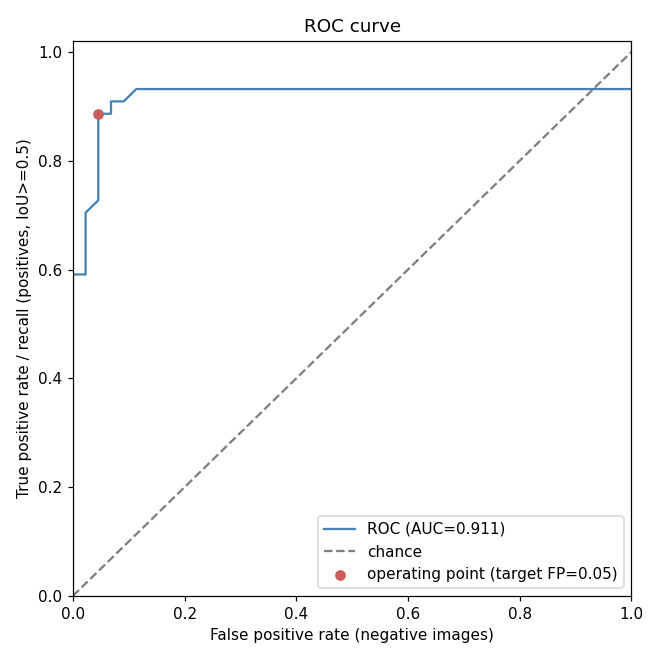
\includegraphics[width=0.38\linewidth]{figures/roc_curve_eval_results_final_test.png}
\hspace{0.5cm}
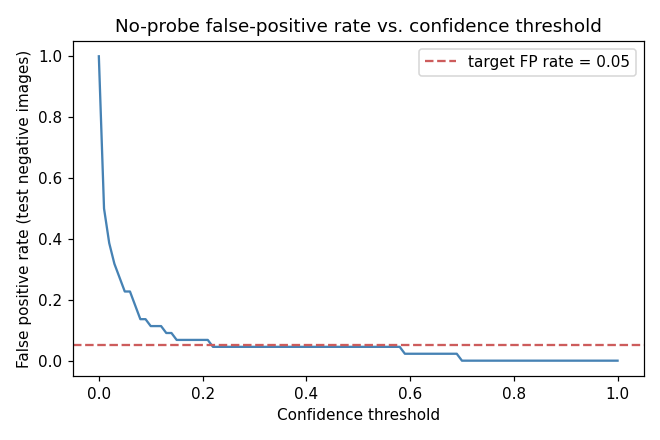
\includegraphics[width=0.38\linewidth]{figures/fp_rate_vs_threshold_eval_results_final_test.png}
\caption{Held-out test curves. Left: ROC curve for probe/no-probe discrimination. Right: false-positive rate on synthetic no-probe images as the confidence threshold changes.}
\end{figure}

The test result is slightly lower than validation AP@0.5 (0.951 vs. 0.964), but the gap is modest. An arbitrary high threshold (e.g. $\tau \ge 0.50$) would cause severe false negatives in challenging flight conditions (low light, glare, steep angles). Conversely, the validation curve shows that background noise peaks below $0.20$. Explicitly selecting the calibrated floor \textbf{$\tau = 0.22$} maximizes probe recovery (recall 0.886 vs. 0.841 at 0.35) while maintaining false alarms on probe-free scenes strictly below the 5\% target (0.045).

\section{Inference, limitations and future improvements}

\texttt{inference.py} accepts a folder of images, draws the highest-confidence probe box when it exceeds the default calibrated threshold of $\tau = 0.22$ (configurable via \texttt{--conf}), and otherwise explicitly marks ``No probe detected''. It saves annotated images and a machine-readable \texttt{detections.json} file.

The most relevant limitation is that no real probe-free frame was available: false-positive behaviour is measured on inpainted rather than naturally negative images. Additional flights, devices, surfaces and real no-probe frames would make both the threshold calibration and generalization claim stronger.

\textbf{Performance and robustness improvements}:
\begin{itemize}[nosep]
    \item \textbf{Spatial Position Prior}: The probe is mechanically constrained to fixed mounting zones on the Elios3 frame (top or bottom of the image). Encoding this prior during training (e.g.\ custom anchor placement or RoI cropping) could improve recall and suppress out-of-bounds false positives. Omitted due to time constraints.
    \item \textbf{Group K-Fold Cross-Validation}: With only 5 drones and 21 flight sequences, a single train/val/test split may not capture the full variance. A grouped K-Fold scheme rotating flight groups across folds would yield a more robust estimate of generalization performance. Collecting real probe-free flights would further strengthen false-positive calibration.
\end{itemize}

\textbf{Inference runtime improvements for IoT deployment}:
\begin{itemize}[nosep]
    \item \textbf{Model quantization}: The model weights can be converted from 32-bit to 16-bit or 8-bit precision, reducing memory usage and significantly increasing inference speed on embedded GPU boards.
\end{itemize}

\section*{Tools and AI Assistance}
Training was executed on Google Colab. AI-assisted coding tools (OpenAI Codex, Anthropic Claude, Google Gemini) were used during development.

\end{document}






